\documentclass[a4paper,10pt]{article}

\usepackage[T1]{fontenc}
\usepackage[utf8]{inputenc}
\usepackage{multicol}
\usepackage{upgreek}
\usepackage{color}
\usepackage{amsmath}
\usepackage{amsfonts}
\usepackage{amssymb}
\usepackage{graphicx}
\usepackage[bottom]{footmisc}
\usepackage{multirow}
\usepackage[english]{babel}
\usepackage{float}
\usepackage[hang]{caption}
\usepackage{subfig}
\usepackage[pdftex]{hyperref}
\hypersetup{colorlinks=false,pdfborder={0 0 0}}
\usepackage[a4paper]{geometry}


\newcommand{\depth}{9}
\newcommand{\mktit}{
	\thispagestyle{empty}
	\begin{center}
	%\includegraphics[height=0.2\textheight]{./photos/lattice} \\
	\hrulefill \\
	\begin{huge}Contact Potential Difference and Photo Voltage \\ \end{huge} 
	\begin{Large} Comparing the Kelvin Probes \\ \end{Large} \vspace*{0.8cm}

	\begin{large}Timo Bretten  \\\end{large} \vspace*{1.2cm}	
	
	\today \\ \vspace*{0.8cm}
	\begin{LARGE}For the Cahen group\\\end{LARGE}
	
	%\includegraphics[height=0.45\textheight]{./photos/dia}
	\end{center}
	\newpage
	\setcounter{page}{2}
}

\newcommand{\sih}{Si--H}
\newcommand{\wfp}{\ensuremath{\upvarphi _{\text{Probe}}}}
\newcommand{\wfs}{\ensuremath{\upvarphi _{\text{Sample}}}}
\newcommand{\cpd}{\text{CPD}}
\newcommand{\McA}{Mc Allister}
\newcommand{\hopg}{HOPG}
\newcommand{\kp}{KP}
\newcommand{\spv}{SPV}

\begin{document}
\mktit

\section{Introduction}
The purpose of this manual is to outline the measurements I did to compare the three Kelvin Probes (\kp{}s) in 618, 301 and 101. The one i 618 measures in ambient, 301 in the glovebox (=nitrogen atmosphere) and the one inside the Lakeshore in 101 (referred to as the \McA{}) can measure in ambient, under vacuum and with temperature dependence. Next to measuring the contact potential difference (\cpd{}), all three \kp{}s can be used to illuminate a sample and thus measure the surface potential volage (\spv{}).\\
A standard reference with known and stable work-function, \hopg{}, is used to callibrate the probe, to find the workfunction of the probehead. To compare the three probes, I used \sih{} as a relatively stable and well understood sample. The results of this comparison will be summarised in Section \ref{sec:results}.
\subsection{(Brief-)Theory}

\section{Procedure}

\subsection{\sih{} Sample Preparation}
n-\sih <100> is prepared according to a slightly modified standard procedure:
\begin{itemize}
	\item Cut, wipe with Ethyl Acetate, Rinse with Ethyl Acetate
	\item Sonicate for 6 min each in Ethyl Acetate, Acetone, Ethanol and Water. Rinse with new solvent before sonication.
	\item Blow dry with $N_2$
	\item Asher for 3 min at 100W; 1l/min $O_2$; 1l/min $Ar$
	\item Etch in 2\% HF for 1 min
	\item repeat Asher
	\item repeat Etch
\end{itemize}
During the last etch, take a stopwatch and let it run upward from zero, bring it with you to the KP and record the time between takind the sample out of the etch and the beginning of the CPS measurement.
 
\subsection{Callibration}
The aim of the callibration is to find the workfunction of the probe \wfp.\\
Take a piece of \hopg{}, put it on the sample holder. Take a piece of scoth tape and tape the \hopg{} down on the holder. Gently and uniformly secure the tape onto \hopg{} with tweezers. Rip off the tape, a smooth surface of \hopg{} should be left behind. Mount this onto a sample holder, measure the \cpd{}.\\
In 618 and 301 the \cpd{} is given as:
\begin{equation}
\cpd  \, = \, \wfs - \wfp \, ,
\end{equation}
so $\wfp = \wfs + \cpd$, so the value for the probe is given as  $\wfp = 4.65 - \cpd$. For the \McA, the equation depends on the way you connect the setup. Here, the equation is:
\begin{equation}
\cpd  \, = \, \upvarphi _{\text{Pre-Amp}} - \upvarphi _{\text{Other}} \, .
\end{equation}
Most often, the pre-amp will be connected to the probe-head, so its workfunction will be given by $\wfp = 4.65 + \cpd$.\\
\hopg{} will deteriorate in air with time. Most probably, this is due to water adsorption on the surface. It is therefore adviseable to be quick with the measurement, not to wait till stabilisation and average only the first few points.

\subsection{\sih{} Measurement}
Measure the \cpd{} of \sih{} for at least two minutes. Change the position of the probehead over the sample, measure again for at least two minutes, repeat. The stopwatch used to time the etch should be running continuously. In this way, the sample's exposure time to air for each individual \cpd{} measurement is known. When analysing the data, a plot of \cpd{} vs time should yield a (more or less) straight line. The y-intercept of that line is (close to) the actual \cpd{}-value that would have been measured immediately after the etch, i.e. for a perfectly fresh surface.

\section{Results}
	\label{sec:results}

\subsection{\hopg{}}
As mentioned, \hopg{} deteriorates slowly in air. The change in \cpd{} is $-1.0 \pm 0.1 \frac{mV}{min}$, consistent in 618 and the \McA{} so it might well happen that HOPG doesn't 'stabilise'~\footnote{Our definition of 'stable' is: standard deviation $<0.5$, $\frac{d(\cpd{})}{dt}<1\frac{mV}{min}$}.\\
In the \McA{}, a jump of 20-40 mV can be observed when switching on the weak pump and a similar jump of $\sim$10 mV is often observed when switching on the turbo pump. The best explanation for this is a displacement of the probe head over the sample, since the jumps are inconsistent in size and birection but always within the known inhomogeinity of \hopg{}.  The \cpd{} of \hopg{} is independent of temperature to within 10 mV, measured over a range of 50K to room-temperature, in steps of 50K.\\
\hopg{} cleaved within the glovebox gives a $\sim$60mV lower \cpd{} than \hopg{} cleaved outside, but their margins of error overlap and that difference is thus not significant.

\subsection{\sih{}, Si-alumina and Si-aluminium}
n-Silicon-H was prepred and measured according to the procedure outlined above. The results of that comparison are given in Figure \ref{fig:nsih}.
\begin{figure}
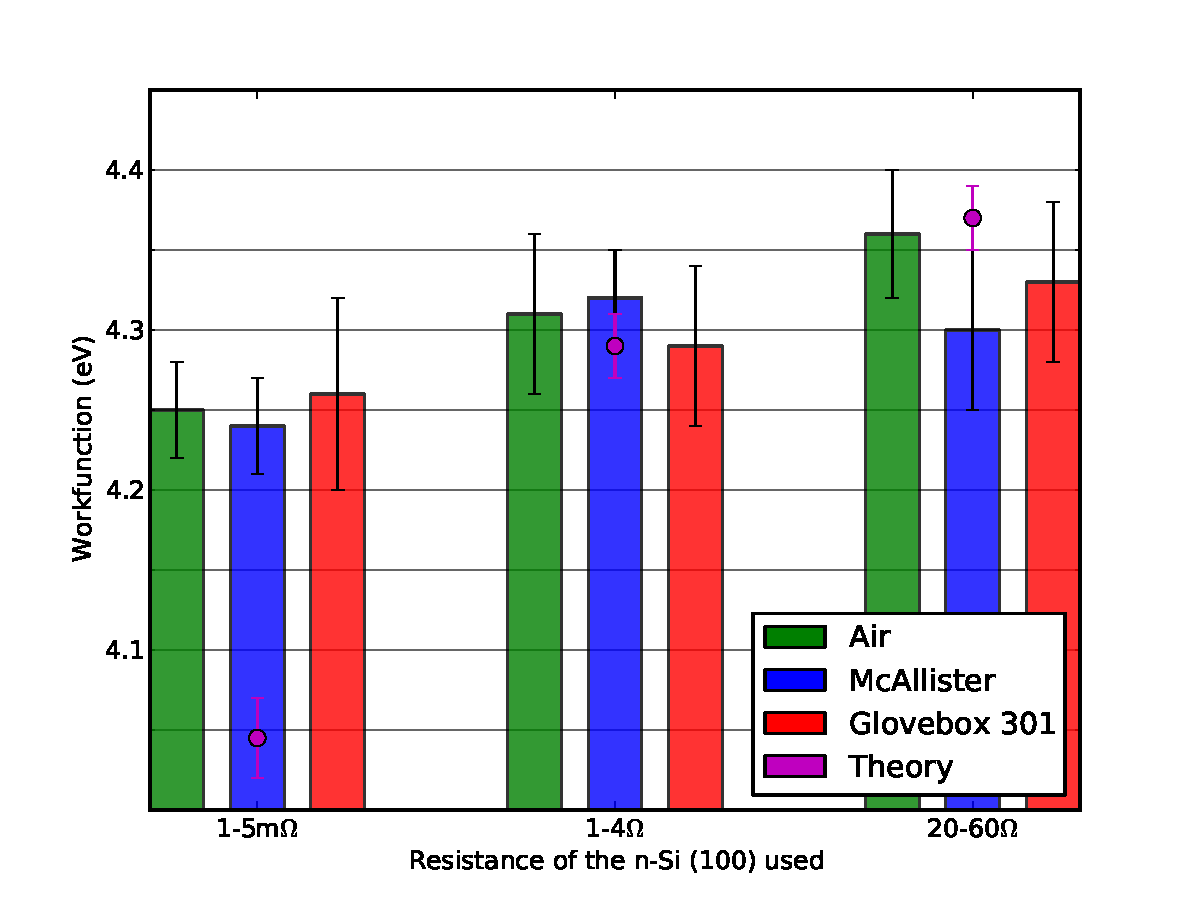
\includegraphics[width=1\textwidth]{Sih}
\caption{Summary of the measured workfunction for the n-\sih{} samples used, compared to theoretically expected values. The indicated error includes deviations in the samples as well as the inaccuracy of callibration with \hopg{}.}
\label{fig:nsih}
\end{figure}
All Kelvin Probes give the same results within the margin of error of the measurement. The relatively large deviation from theory for low-resistivity, highly-doped Silicon is probably due to the wafer being very old or even mislablled.\\
The McA\{} was compared to the \kp{} in 618 also with an alumina passivated sample of Silicon. 
\end{document}
